%! Author = antoniomasotti
%! Date = 25.11.23


\begin{frame}{Contracts}

    \begin{block}{Contracts}
        A formal agreement between parties or individual. Synonyms: agreement, protocol, deal

        --- Oxford English Dictionary
    \end{block}

\end{frame}

\begin{frame}{Contract Test Role}
    \begin{center}
            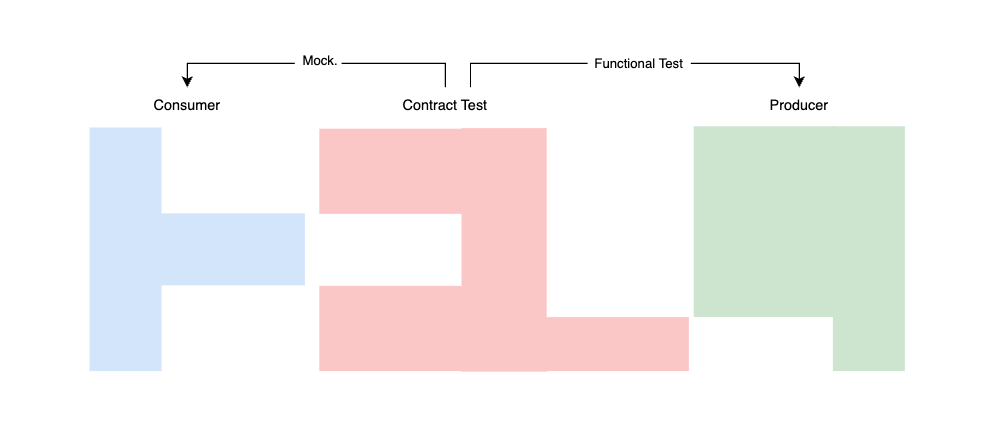
\includegraphics[scale=.3]{./assets/contract_divided}
            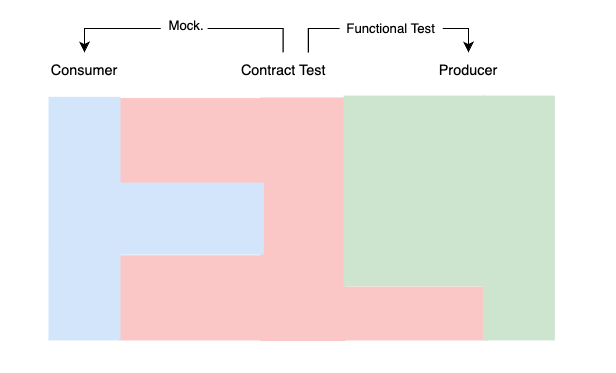
\includegraphics[scale=.3]{./assets/contract_united}
    \end{center}
\end{frame}

\subsection{Pact}

\begin{frame}{Pact - Consumer Driven Contracts}
    "`\textit{A strange inversion of reasoning...}"'
    \begin{columns}
        \begin{column}{0.5\textwidth}
            \begin{itemize}
                \item Consumer Driven Contracts
                \item Pact is a contract testing tool
                \item Pact is a specification for consumer driven contracts
                \item Pact is a set of frameworks that support consumer driven contracts
            \end{itemize}
        \end{column}
        \begin{column}{0.5\textwidth}
            \begin{center}
                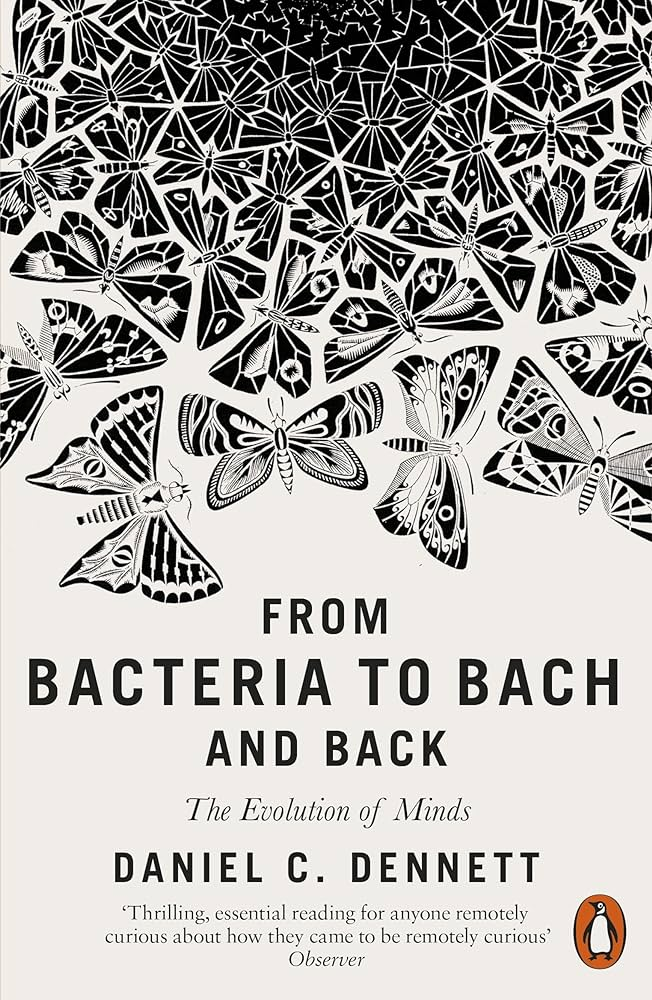
\includegraphics[width=.5\textwidth]{./assets/bacteria}
                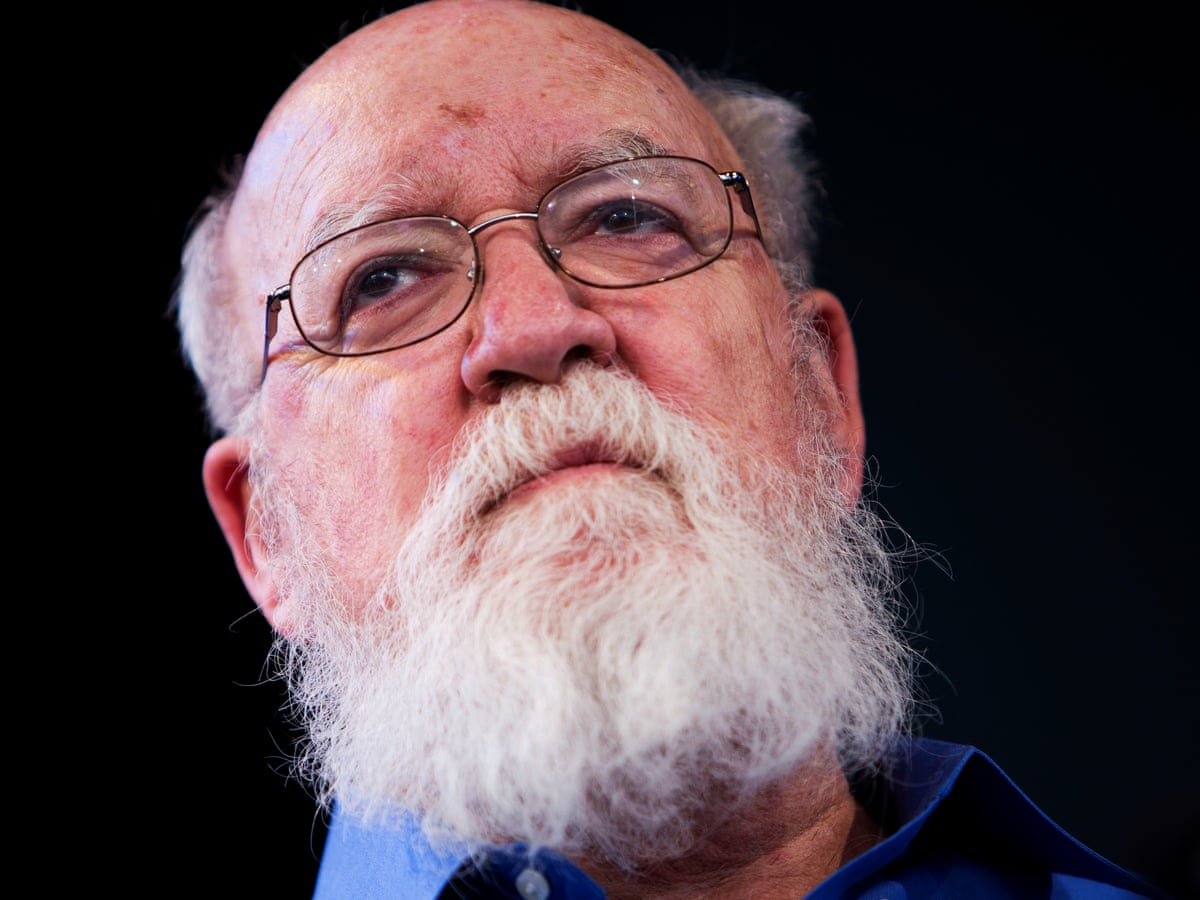
\includegraphics[width=.5\textwidth]{./assets/dennet}
            \end{center}
        \end{column}

    \end{columns}
\end{frame}
